\documentclass{article}


% if you need to pass options to natbib, use, e.g.:
%     \PassOptionsToPackage{numbers, compress}{natbib}
% before loading neurips_2025

\PassOptionsToPackage{numbers, compress}{natbib}

% ready for submission
\usepackage{neurips_2025}


\bibliographystyle{abbrvnat}

\usepackage[pdftex]{graphicx}
\usepackage{amsmath}
% to compile a preprint version, e.g., for submission to arXiv, add add the
% [preprint] option:
%\usepackage[preprint]{neurips_2025}


% to compile a camera-ready version, add the [final] option, e.g.:
%     \usepackage[final]{neurips_2025}


% to avoid loading the natbib package, add option nonatbib:
%    \usepackage[nonatbib]{neurips_2025}


\usepackage[utf8]{inputenc} % allow utf-8 input
\usepackage[T1]{fontenc}    % use 8-bit T1 fonts
\usepackage{hyperref}       % hyperlinks
\usepackage{url}            % simple URL typesetting
\usepackage{booktabs}       % professional-quality tables
\usepackage{amsfonts}       % blackboard math symbols
\usepackage{nicefrac}       % compact symbols for 1/2, etc.
\usepackage{microtype}      % microtypography
\usepackage{xcolor}         % colors

\newcommand\reynotes[1]{\textcolor{purple}{#1}}

%\title{SmokeViz: Using Pseudo-Labels to Develop a Human-Labeled Deep Learning Dataset of Wildfire Smoke Plumes in Satellite Imagery}
\title{SmokeViz: A Large-Scale Satellite Dataset for Wildfire Smoke Detection and Segmentation}


% The \author macro works with any number of authors. There are two commands
% used to separate the names and addresses of multiple authors: \And and \AND.
%
% Using \And between authors leaves it to LaTeX to determine where to break the
% lines. Using \AND forces a line break at that point. So, if LaTeX puts 3 of 4
% authors names on the first line, and the last on the second line, try using
% \AND instead of \And before the third author name.


\author{%
  Rey Koki\\%\thanks{rey.koki@colorado.edu} \\
  Department of Computer Science\\
  University of Colorado Boulder\\
  Boulder, Colorado 80303\\
  \texttt{rey.koki@colorado.edu} \\
  % examples of more authors
  % \And
  % Coauthor \\
  % Affiliation \\
  % Address \\
  % \texttt{email} \\
  % \AND
  % Coauthor \\
  % Affiliation \\
  % Address \\
  % \texttt{email} \\
  % \And
  % Coauthor \\
  % Affiliation \\
  % Address \\
  % \texttt{email} \\
  % \And
  % Coauthor \\
  % Affiliation \\
  % Address \\
  % \texttt{email} \\
}


\begin{document}


\maketitle


\begin{abstract}
    The global rise in wildfire frequency and intensity over the past decade underscores the need for improved fire monitoring techniques. To advance deep learning research on wildfire detection and its associated human health impacts, we introduce \textbf{SmokeViz}, a large-scale machine learning dataset of smoke plumes in satellite imagery. The dataset is derived from expert annotations created by smoke analysts at the National Oceanic and Atmospheric Administration, which provide coarse temporal and spatial approximations of smoke presence. To enhance annotation precision, we propose \textbf{pseudo-label dimension reduction (PLDR)}, a generalizable method that applies pseudo-labeling to refine datasets with mismatching temporal and/or spatial resolutions. Unlike typical pseudo-labeling applications that aim to increase the number of labeled samples, PLDR maintains the original labels but increases the dataset quality by solving for intermediary pseudo-labels (IPLs) that align each annotation to the most representative input data. For SmokeViz, a parent model produces IPLs to identify the single satellite image within each annotations time window that best corresponds with the smoke plume. This refinement process produces a succinct and relevant deep learning dataset consisting of over 180,000 manual annotations. The SmokeViz dataset is expected to be a valuable resource to develop further wildfire-related machine learning models and is publicly available at \url{https://noaa-gsl-experimental-pds.s3.amazonaws.com/index.html#SmokeViz/}.
\end{abstract}


\section{Introduction}

Due in part to public policy, average fine particulate matter (PM\textsubscript{2.5}) levels in the United States have declined over recent decades \cite{clean_air_act}. However, from 2010 to 2020, the contribution of wildfire smoke to PM\textsubscript{2.5} concentrations more than doubled, accounting for up to half of total PM\textsubscript{2.5} exposure in Western U.S. \cite{smoke_PM}. This is particularly concerning, as ambient PM\textsubscript{2.5} is a leading environmental risk factor for adverse health outcomes and premature mortality \cite{smoke_mortality}. These trends/risks highlight the urgent need for scalable and timely smoke monitoring systems to mitigate public health risks.

Satellite imagery offers the spatial coverage and temporal frequency needed for large-scale smoke monitoring. In comparison to polar-orbiting satellites like Suomi or Sentinel, Geostationary satellites such as the GOES series \cite{goes} are especially well-suited to this task, providing persistent observation over fixed regions—essential for capturing the dynamic behavior of wildfire smoke plumes. The high temporal resolution and wide coverage of GOES imagery enable real-time tracking of smoke concentration and movement, supporting air quality assessments and early warning systems.

Even with the advances in remote sensing, existing deep learning satellite datasets for wildfire smoke detection face several limitations. They are often small in scale, restricted to specific regions or events, and focus on scene-level classification rather than pixel-level segmentation. Most do not differentiate between smoke density levels, are not publicly available, and lack standardized benchmarks for semantic segmentation. While NOAA’s Hazard Mapping System (HMS) provides a large-scale, expert-labeled dataset, its annotations span multi-hour time windows that vary in duration. This creates a temporal mismatch between the labels and individual satellite frames, complicating their direct use for supervised learning.

To address these challenges, we introduce \textbf{SmokeViz}, a large-scale satellite dataset for semantic segmentation of wildfire smoke plumes. SmokeViz includes over 180,000 annotated samples derived from GOES-East and GOES-West imagery, aligned with HMS analyst annotations. To resolve the temporal ambiguity in the original labels, we propose a semi-supervised method called \textbf{pseudo-label dimension reduction (PLDR)}, which uses intermediary pseudo-labels to select the satellite image that best matches each smoke annotation. The resulting dataset provides one-to-one image-to-label pairs with ordinal smoke density masks, suitable for supervised deep learning.

\textbf{SmokeViz} serves as a benchmark for wildfire smoke segmentation and as a resource for the broader machine learning community working with geospatial, temporal, and remote sensing data. It supports new directions in ordinal segmentation, semi-supervised learning with temporal uncertainty, and pretraining for Earth observation tasks involving dynamic atmospheric phenomena.

\textbf{Our contributions are:}
\begin{itemize}
    \item We introduce \textbf{SmokeViz}, the largest satellite-based dataset for wildfire smoke segmentation, with over 180,000 samples from GOES imagery.
    \item We propose \textbf{PLDR}, a physics-guided semi-supervised method for aligning coarse human annotations with temporally optimal satellite imagery.
    \item We provide benchmark segmentation baselines and standardized training splits to support reproducibility and downstream research.
\end{itemize}

\section{Related Work}

\subsection{Smoke Detection and Labeling Methods}

Multi-channel thresholding remains a widely used method for distinguishing smoke from similar atmospheric signatures such as dust or clouds using channel-specific radiance values \cite{threshold}. These thresholds are typically derived from labeled historical data and are fine-tuned to specific regions and fuel types, limiting their generalizablity \cite{thresh_geog}. In contrast, the SmokeViz dataset spans a wide range of biogeographies across North America and can serve as a source of refined analyst-labeled examples for developing more generalizable thresholding techniques.

Large parameterized numerical models are used for forecasting smoke dispersion, but not for smoke detection itself. Systems such as HRRR-Smoke and RRFS \cite{hrrr, rrfs} rely on computationally intensive forecasts requiring nearly 200 dynamic meteorological inputs. A key limitation of these models is the absence of a real-time smoke analysis product for data assimilation, resulting in delayed model spin-up and compounded forecast errors. Model predictions from SmokeViz could help fill this gap, offering a real-time, satellite-driven alternative to support data assimilation for operational smoke dispersion forecasting.

Manual smoke labeling is performed by trained analysts through visual inspection of satellite imagery. NOAA’s Hazard Mapping System (HMS) provides a analyst-labeled wildfire smoke dataset \cite{hms, hms_val}. HMS analysts examine GOES imagery sequences to track smoke plume movement and annotate the approximate spatial extent and qualitative density of smoke (light, medium, heavy), as illustrated in Figure~\ref{densities}. Annotations are issued on a rolling basis and span time windows ranging from instantaneous to over 20 hours \cite{hms_web}. While HMS provides high-quality expert annotations, its operational format introduces challenges for supervised learning: annotations are temporally coarse, vary in length, and lack one-to-one correspondence with satellite frames. SmokeViz refines HMS annotations into temporally resolved, frame-aligned labels, enabling real-time, continuous predictions of smoke extent and density.

\begin{figure}[!htb]
    \centering
    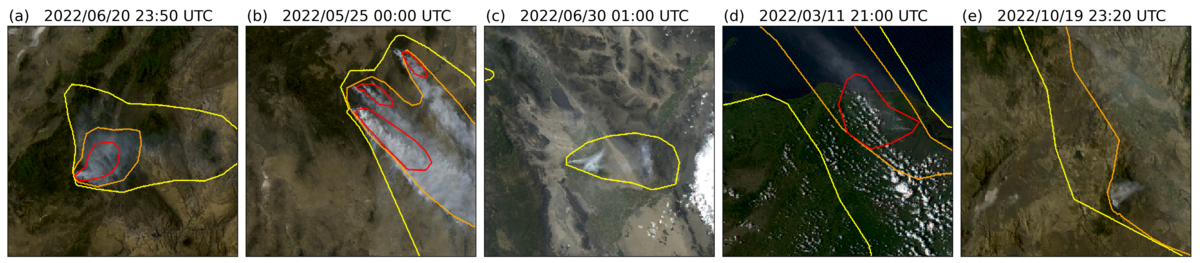
\includegraphics[width=\linewidth]{figures/variations_small.png}\label{densities}
    \caption{HMS smoke annotations overlaid on GOES imagery. Yellow, orange, and red contours indicate light, medium, and heavy smoke density, respectively. (a) and (b) show canonical smoke plumes; (c)–(e) illustrate density label variation across scenes.}
\end{figure}

\subsection{Deep Learning Datasets and Models for Wildfire Smoke}

Recent efforts have applied deep learning to wildfire smoke detection using a variety of satellite sources and label strategies. SmokeNet \cite{smokenet} employs a convolutional neural network (CNN) to classify MODIS image scenes as containing smoke or not, using student-provided labels. SatlasPretrain \cite{satlas} includes a small set of Sentinel-2 images labeled for smoke as part of a larger multi-label pretraining dataset. While scene classification methods can provide wildfire detection information, they do not capture spatial characteristics of smoke plumes that segmentation would be more appropiate to capture.

Several datasets have been developed for smoke segmentation, but they are limited in scope. Wen et al.\ \cite{smoke_goes} trained a CNN on GOES-East imagery over California and Nevada using HMS annotations from the 2018 wildfire season. Larsen et al.\ \cite{larsen} used Himawari-8 data to detect smoke at the pixel level for a single fire event, using a threshold-based algorithm as ground truth. Table~\ref{studies} compares these datasets in terms of scale, source, and labeling. SmokeViz stands out by offering over 180,000 samples with analyst-generated, frame-aligned labels covering multiple fire seasons, regions, and biogeographies. It is, to our knowledge, the largest and most diverse dataset for smoke plume segmentation.


\begin{table*}[h]
    \caption{Comparison of satellite smoke plume datasets, detailing the number of smoke plume samples, satellite source, number of spectral bands, labeling method, classification type - scene classification (SC) or semantic segmentation (SS), and public availability.}\label{studies}
    \centering
    \begin{tabular}{ccccrrcrc}
        \toprule
        reference & \verb|#| samples & satellite & \verb|#| bands & label & task & avail.\\
        \midrule
        \cite{smokenet}& 1016 & MODIS & 5 & students & SC & no \\
        \cite{satlas} & 125 & Sentinel-2 & 3 & crowd sourced & SC & yes \\
        \cite{smoke_goes}& 4095 & GOES-East & 5 & HMS analysts & SS & no \\
        \cite{larsen} & 975 & Himiwari-8 & 7 & algorithm& SS & no \\
        %\cite{wang}& 47 & Landsat-8 & 4 & & \\
        SmokeViz  & 183,672 & GOES-East/West & 3 & HMS analysts & SS & yes \\
        \bottomrule
    \end{tabular}
\end{table*}

In addition to its relevance for wildfire applications, SmokeViz contributes a challenging benchmark for general-purpose remote sensing vision tasks. Unlike many existing datasets that avoid cloudy scenes \cite{bigearthnet, crops} or focus on sharply bounded features such as cropland \cite{crops}, infrastructure \cite{polyworld}, or oceanic clouds \cite{cyclone, cloud_texture}, smoke has amorphous, fading boundaries in both space and time. Incorporating smoke segmentation into large-scale pretraining corpora, such as SatlasPretrain \cite{satlas}, could enhance generalizable models for Earth observation.

\subsection{Pseudo-labeling}

Semi-supervised learning techniques such as pseudo-labeling have been widely used to expand training data by leveraging unlabeled samples \cite{pseudo}. Typically, a parent model is trained on labeled data and then used to generate pseudo-labels for an unlabeled dataset, which are in turn used to train subsequent models in an iterative process.

In contrast, we propose a non-iterative variation focused not on data expansion, but dataset data-to-label precision. Our method, \textbf{pseudo-label dimension reduction (PLDR)}, generates intermediary pseudo-labels (IPLs) for each satellite frame within the HMS annotation window. Rather than using these labels for training, we use them to identify the satellite image with the greatest alignment to the analyst annotation. This enables the construction of SmokeViz, a temporally disambiguated, one-to-one image-to-label dataset. The resulting dataset methodically pairs the analyst-generated smoke plume labels with selected GOES imagery, enabling high-resolution, temporally accurate segmentation model training.


\section{Methods}
\subsection{Datasets}

We use imagery from the latest GOES satellites, GOES-16 (East), GOES-17 and GOES-18 (West), each equipped with the ABI, which captures 16 spectral bands from visible to infrared wavelengths (\(\lambda\)s) every 10 minutes. We process bands 1-3 using \texttt{PyTroll} \cite{satpy} to generate 1km true-color composites \cite{true_color}, matching the composite viewed by HMS analysts. These bands correspond to the shortest \(\lambda\)s available on ABI and yield the highest signal-to-noise ratio (SNR).

To leverage movement characteristics of smoke, HMS analysts use multi-frame animations of the satellite imagery. The time windows are defined by  approximate number of frames the analyst views smoke, often with buffers before the fire starts. Annotations span varying time windows, often covering multiple hours, averaging three hours per annotation. Since the HMS annotations are designed to reflect overall plume extent during a time window rather than at any specific moment, smoke boundaries in individual frames may not align well with the annotation (Figure \ref{timelapse}). A naive modeling approach would use all frames within each time window as input, but this introduces non-uniform sequence lengths and significantly increases memory and computational demands, which complicates the use of deep learning architectures and model usage in real-time operations. Instead, we establish a one-to-one mapping by identifying the single satellite frame that best matches each analyst annotation.

\begin{figure}[!htb]
    \centering
    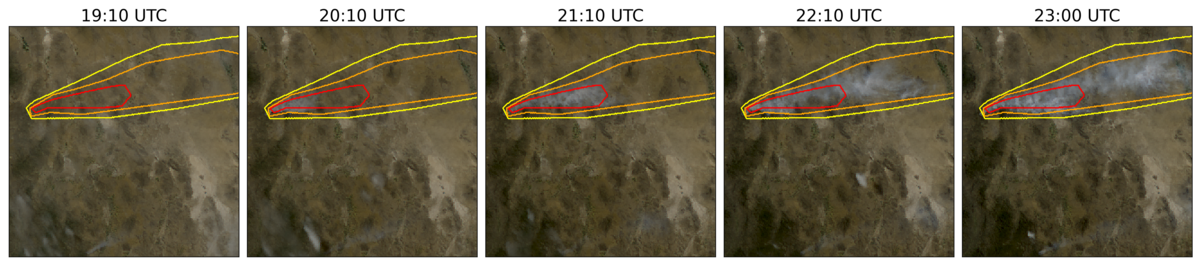
\includegraphics[width=\linewidth]{figures/timelapse_small.png}
    \caption{True color GOES-East imagery from May 5th, 2022, Southeast New Mexico (\(31.38^{\circ}\)N, \(107.87^{\circ}\)W) during the start of the Foster Fire. The red, orange and yellow lines represent the heavy, medium and low density HMS smoke annotations that span 19:10\textendash23:00 UTC.}
    \label{timelapse}
\end{figure}


We select either GOES-East or GOES-West based on the solar zenith angle (SZA) to optimize for forward Mie scattering. For smoke identification, this approach can achieve a much higher SNR than imaging the earth’s surface from an arbitrary angle. While the atmosphere is composed primarily of molecules with size \(<\)1nm, smoke particles are larger in comparison, varying from 100 nm -- 10 \(\mu\)m in diameter, \(d\). When the \(\lambda\) of light \(\lambda<d\), the elastic scattering of light against matter is modeled through Mie rather than Rayleigh scattering (Figure \ref{mei}). Therefore, smoke observation favors forward scattering and short \(\lambda\) so that we select (1) the satellite that would observe the most Mie forwad scattering as demostrated in Figures \ref{WEST_EAST_bands}(a) vs \ref{WEST_EAST_bands}(b) that show GOES-East displaying a higher SNR near sunset compared to GOES-West. (2) the three shortest \(\lambda\) ABI bands (C01-C03: 0.47, 0.64, and 0.865\(\mu\)m) that give the highest smoke SNR as seen in Figures \ref{WEST_EAST_bands}(c)-\ref{WEST_EAST_bands}(e).


\begin{figure}[!htb]
    \centering
    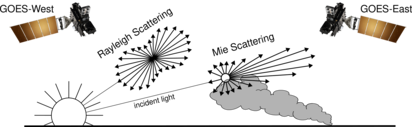
\includegraphics[width=8cm]{figures/mei_small.png}
    \caption{If the particle size is \(<\frac{1}{10}\) the \(\lambda\) of the interacting light, then the primary scattering will be Rayleigh. Mie scattering is the predominant scattering mechanism when the particle size is larger than the \(\lambda\) of light. This schematic demonstrates that when the sun is setting in the West, the Mie scattering will predominately forward scatter towards GOES-East.} \label{mei}
\end{figure}

\begin{figure}[!htb]
    \centering
    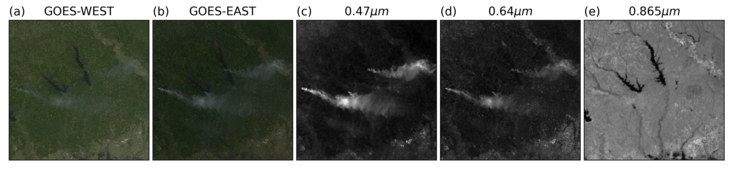
\includegraphics[width=\linewidth]{figures/GOES_WEST_EAST_B_R_V_small.png}
    \caption{True color (a) GOES-WEST and (b) GOES-EAST imagery from March \(23^{rd}\), 2022 centered at (\(31.1^{\circ}\), \(-93.8^{\circ}\)) in Texas, USA taken at 23:20 UTC. The GOES-EAST raw band imagery for (c) blue, (d) red and (e) veggie bands show variations in the SNR for smoke detection in relation to the \(\lambda\) of light being measured.}\label{WEST_EAST_bands}
\end{figure}

For the existing dataset of HMS smoke plume annotations and all corresponding satellite imagery, \(\mathcal{D} = \{\mathcal{X}, \mathcal{Y}\}\), for each sample, a label \(y_i \in \mathcal{Y}\) has a set of satellite imagery \([x_{(i,t_0)},...,x_{(i,t_N)}] \in \mathcal{X}\) over the analyst defined time window \(t\). To develop a one-to-one data-to-label dataset, we generate IPLs to develop a subset of \(\mathcal{D}\), denoted as \(\mathcal{D}_p\), that has a one-to-one ratio such that \(|\mathcal{X}_p| = |\mathcal{Y}|\), where we aim to find the satellite image that has the maximum overlap between the geolocation of smoke in the imagery and the analyst annotation using the PLDR method shown in Figure \ref{PLDR}.

\begin{figure}[!htb]
    \centering
    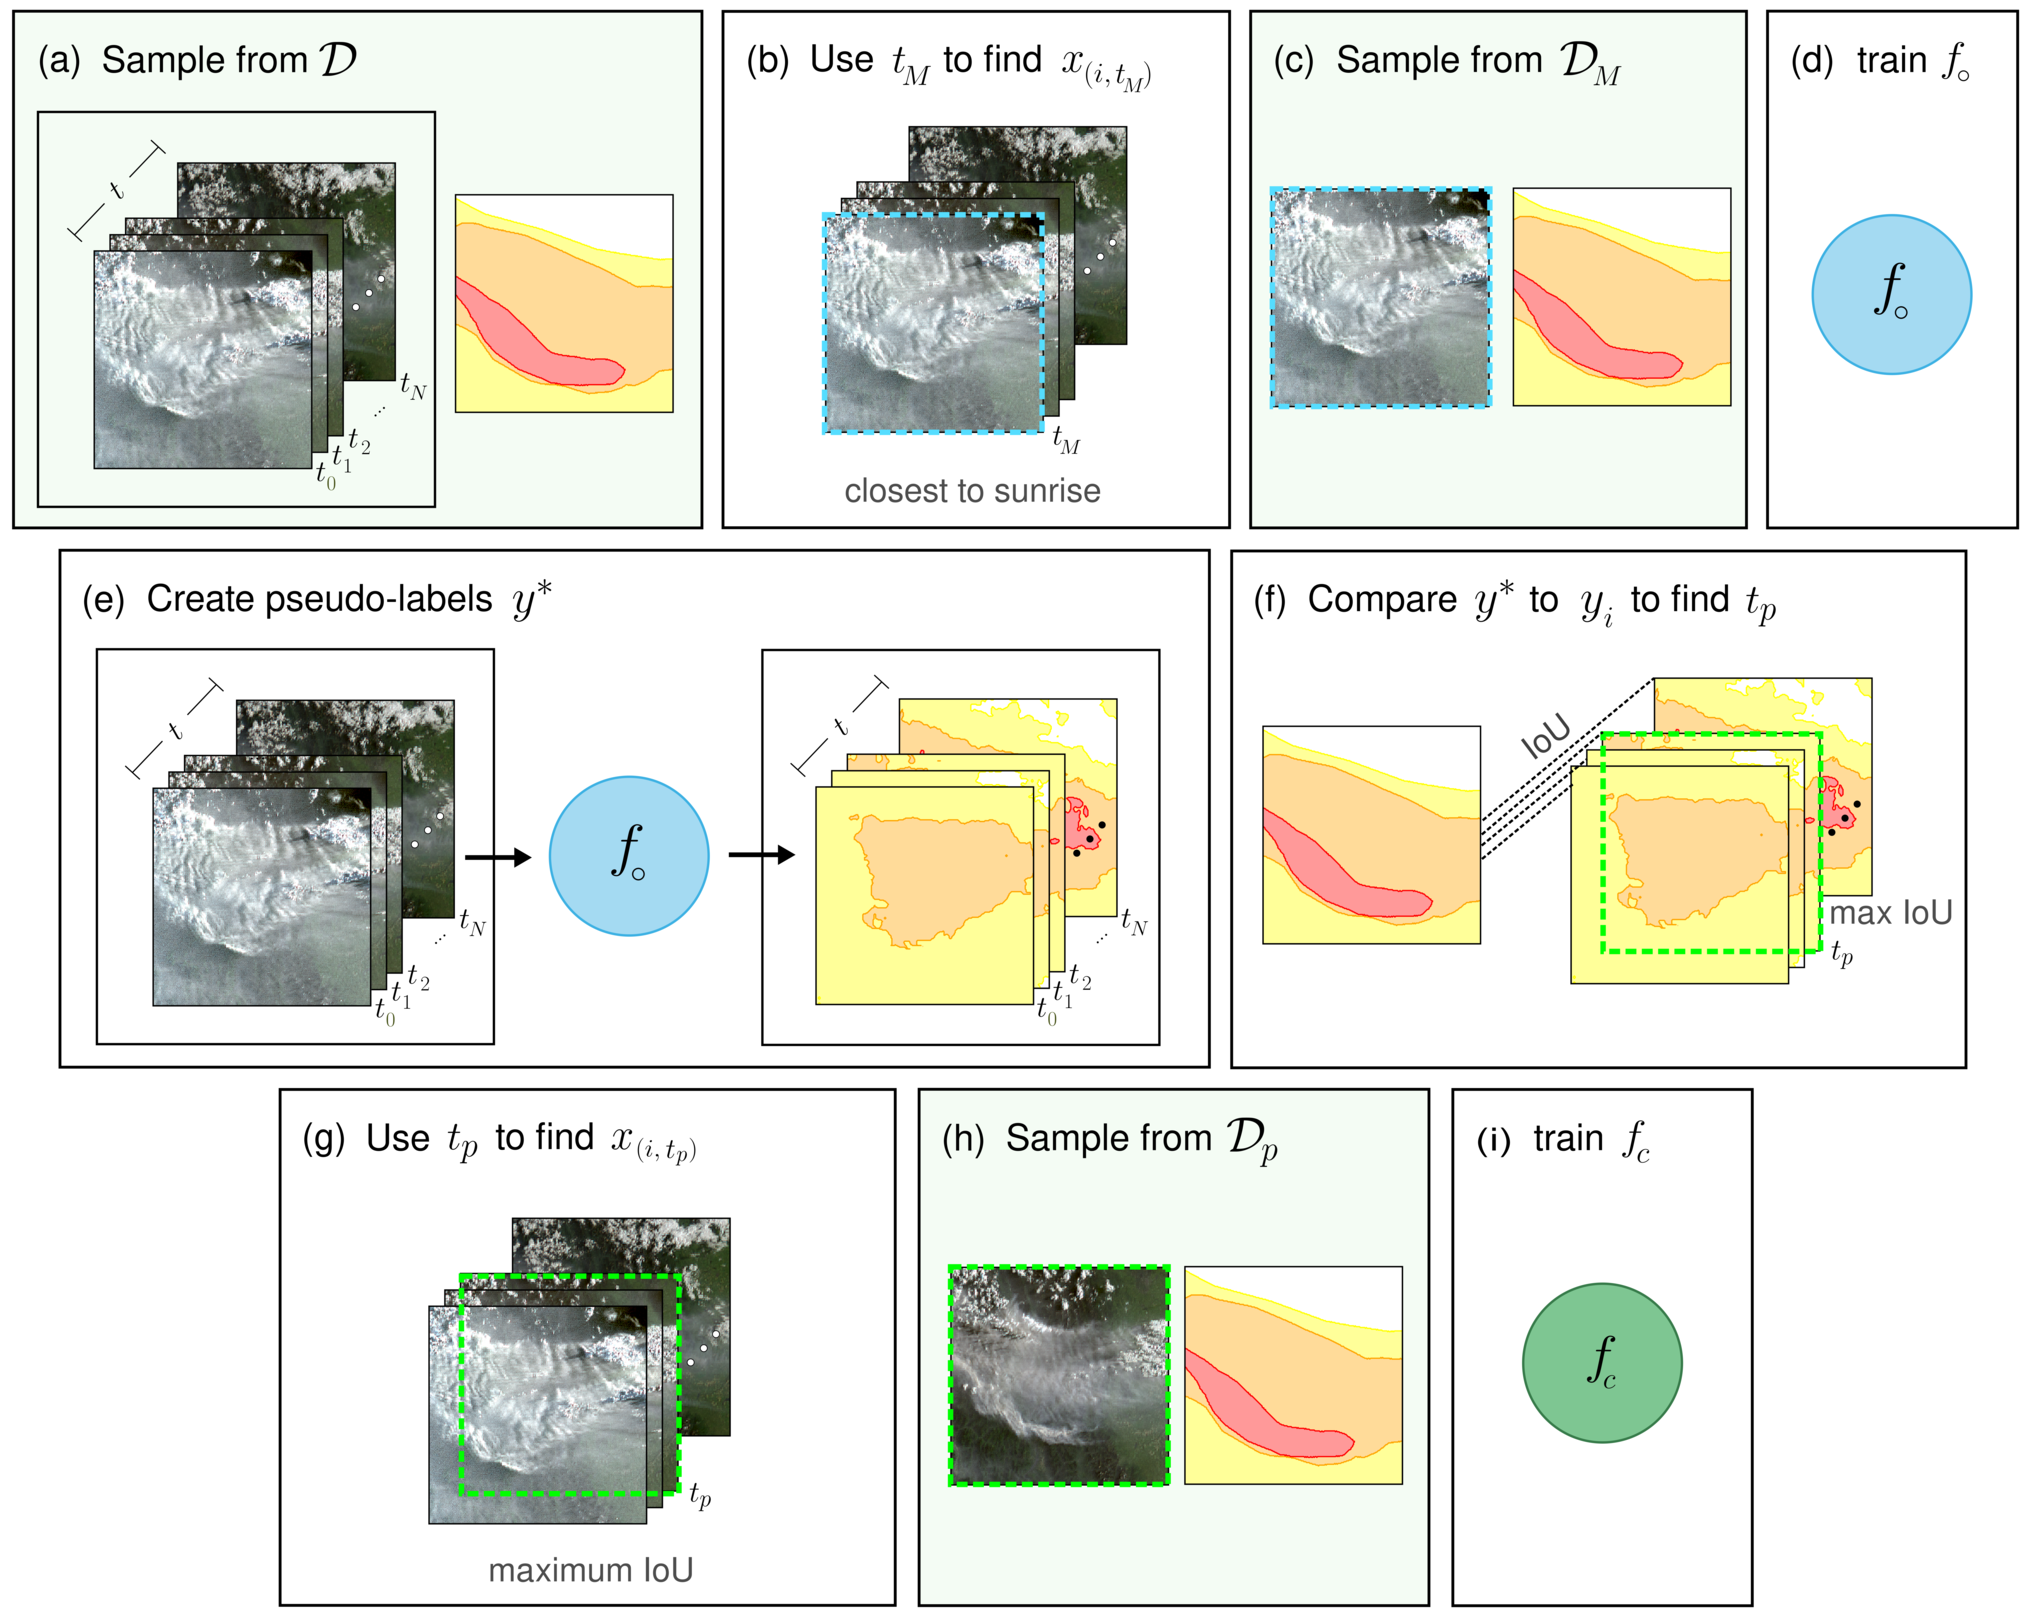
\includegraphics[width=\linewidth]{figures/workflow_small.png}
    \caption{
        PLDR applied to create the SmokeViz dataset. Green boxes indicate dataset stages. 
        (a) For original dataset \(\mathcal{D}\) - analyst annotation \(y_i\) corresponds to \(N\) satellite images across time window \(t\) so that \(([x_{(i,t_0)},...,x_{(i,t_N)}], y_i) \in \mathcal{D}\); 
        (b) use Mie scattering to find the time, \(t_M\), that corresponds with satellite image \(x_{(i,t_M)}\) that would produce the highest possible SNR if smoke was present; 
        (c) resulting \(\mathcal{D}_M\) is one-to-one \((x_{(i,t_M)}, y_i) \in \mathcal{D}_M\);
        (d) parent model \(f_\circ\) is trained; 
        (d) parent model \(f_\circ\) is trained on \(\mathcal{D}_M\) such that \(f_\circ(x_{(i,t_M)})=y_i\);
        (e) apply a greedy algorithm \(f_\circ([x_{(i,t_0)},...,x_{(i,t_N)}])=[y^*_{(i,t_0)},...,y^*_{(i,t_N)}]\) to create IPLs \(y^*\) for each candidate image; 
        (f) compute the intersection over union (IoU) between \(y^*\) and \(y_i\) to identify the time \(t_p\) where the IPL and analyst annotation have the maximum IoU; 
        (g) best match image \(x_{(i,t_p)}\) selected; 
        (g) match \(t_p\) to its correpsonding image \(x_{(i,t_p)}\) that should best match the analyst annotation;
        (h) SmokeViz dataset \(\mathcal{D}_p\) created; 
        (i) child model \(f_c\) is trained on \(\mathcal{D}_p\) such that \(f_c(x_{(i,t_p)})=y_i\) is used to detect and classify the density of wildfire smoke plumes in GOES imagery.
    }
\label{PLDR}
\end{figure}

To train an initial parent model, \(f_{\circ}\), we developed a method of leveraging Mie scattering physics to select \(x_{(i,t_M)} \in \mathcal{X}\) (Figure \ref{PLDR}(b)) so that \(x_{(i,t_M)}\) has a higher chance than random selection out of the set of imagery \([x_{(i,t_0)},...,x_{(i,t_N)}]\) to be representative of \(y_i\). This Mie-Derived Dataset, \(\mathcal{D}_M\) produces a training set so that if there is smoke present during the entire time window, the selected timestamp \(t_M\) would give the highest smoke SNR. 

More importantly than finding the timestamp for maximum the SNR, we want to determine which image actually has smoke present within the smoke label boundaries. We use \(\mathcal{D}_M\) to train \(f_{\circ}\) (Figure \ref{PLDR}(d)), to identify smoke in satellite imagery, and then use that \(f_{\circ}\) to create IPLs of each satellite image in a given annotation's time-window (Figure \ref{PLDR}(e)). From those results, the optimal satellite image is chosen based on which image's IPLs has the greatest overlap with the analyst annotation (Figure \ref{PLDR}(f)-(h)).


\subsubsection{From Full Dataset \(\mathcal{D}\) to Mie-Derived Dataset \(\mathcal{D}_M\)}



Let \(\mathcal{D} = \{\mathcal{X}, \mathcal{Y}\}\) be the original dataset, where each label \(y_i \in \mathcal{Y}\) corresponds to multiple satellite images \([x_{(i,t_0)},...,x_{(i,t_N)}] \in \mathcal{X}\) over a given time window. Using Mie scattering principles, we select the image \(x_{(i,t_M)}\) with the highest expected smoke SNR to form a one-to-one dataset \(\mathcal{D}_M = \{\mathcal{X}_M, \mathcal{Y}\}\) such that \(\mathcal{X}_M \subset \mathcal{X}\) and \(|\mathcal{X}_M| = |\mathcal{Y}|\). The Mie-derived satellite image is chosen based on which frame within the annotation time window would exhibit the strongest forward scattering geometry and thus the highest potential smoke SNR if smoke were present. 

Based on forward scattering criteria, the trivial strategy would be to pull imagery from GOES-West right after sunrise and from GOES-East right before sunset when the SZA is closest to \(90^{\circ}\). However, the time when the SZA approaches \(90^{\circ}\) coincides with when there are maximized atmospheric interactions that cause an increase in noise and artifacts \cite{zen_angle}. To avoid image artifacts caused by extreme SZA, we exclude scenes with SZA \(>88^\circ\) if there are lower SZA images available. The resulting dataset \(\mathcal{D}_M\) contains over 200,000 samples and is used to train the parent model \(f_{\circ}\).

\subsubsection{PLDR Dataset \(\mathcal{D}_p\)} 

\begin{table}
\parbox{.45\linewidth}{
\centering
    \caption{A comparison of how smoke density would be represented by one-hot encoding commonly used for categorical data to thermometer encoding often used for ordinal data.}\label{therm}
    \begin{tabular}{ccccrrcrc}
        \toprule
        density & one-hot & thermometer \\
        \midrule
        none & \texttt{[0 0 0]} & \texttt{[0 0 0]} \\
        light  & \texttt{[0 0 1]} & \texttt{[0 0 1]} \\
        medium & \texttt{[0 1 0]} & \texttt{[0 1 1]} \\
        heavy  & \texttt{[1 0 0]} & \texttt{[1 1 1]} \\
        \bottomrule
    \end{tabular}
}
\hspace{.4cm}
\parbox{.5\linewidth}{
    \caption{Dataset split for \(\mathcal{D}_M\) and \(\mathcal{D}_p\), samples for 2024 go up to November 1st \reynotes{do 2018-2022 instead}. We use an entire year of data for both validation and testing sets to capture year-long wildfire trends.}\label{split}
    \centering
    \begin{tabular}{ccccrrcrc}
        \toprule
        dataset & \(\mathcal{D}_M\) & \(\mathcal{D}_p\) &years\\
        \midrule
        training & 165,609 & 144,225 &2018-22\\
        validation & 20,056 & 19,223 &2023 \\
        testing & 21,541 & 20,224 & 2022 \\
        \bottomrule
    \end{tabular}
}
\end{table}


We train \(f_{\circ}\) on \(\mathcal{D}_M\) (table \ref{split}) to find smoke in GOES imagery. The model is then applied across each satellite image within the time window \([x_{(i,t_0)},...,x_{(i,t_N)}]\) to produce intermediary pseudo-labels (IPLs), \([y^*_{(i,t_0)},...,y^*_{(i,t_N)}]\). We compute the intersection over union (IoU) between each \(y^*\) and the corresponding analyst label \(y_i\), selecting the timestamp \(t_p\) that yields the maximum IoU to define \(\mathcal{D}_p = \{x_{(i,t_p)}, y_i\}\).

\begin{equation} \label{overall_iou}
    IoU_{\text{overall}} = \frac{\sum\limits_{j=\text{light}}^{\text{heavy}}|y_{j}\cap y^*_{j}|}{\sum\limits_{j=\text{light}}^{\text{heavy}}|y_{j}|\cup|y^*_{j}|}
\end{equation}

To build \(f_{\circ}\), we implement \texttt{Segmentation Models PyTorch} \cite{semantic} with EfficientNetV2 \cite{efficientnetv2} as the encoder and PSPNet \cite{pspnet} as the decoder. Input images are \(256\times256\times3\) true-color snapshots; the output is a \(256\times256\times3\) classification map predicting categorical smoke density. We use thermometer encoding to capture the ordinal nature of smoke density classes (Table \ref{therm}) and apply binary cross-entropy loss across the classes. We use a confidence threshold of IoU  >0.01 \cite{conf_thresh} to exclude samples with negligible overlap. 

The same dataset split choices (table \ref{split}) and model setup that were used for \(\mathcal{D}_{M}\) and \(f_{\circ}\) were implemented for to train a child model \(f_c\) on \(\mathcal{D}_p\). To assess if training with \(\mathcal{D}_{p}\) can produce a more robust semantic segmentation model compared to training on \(\mathcal{D}_M\) we run \(f_c\) on the \(\mathcal{D}_{p}\) and \(\mathcal{D}_{M}\) test sets. 

\subsection{Benchmark Models}

We benchmark the SmokeViz dataset \(\mathcal{D}_{p}\) by varying the semantic segmentation architectures. We train Linknet \cite{linknet}, PSPNet \cite{pspnet} and MANet \cite{manet} using the same encoder for \(f_c\) and \(f_{\circ}\), EfficientNetV2. Each model is trained over 100 epochs using a batch size of 32 and the Adam optimizer on 8 16GB memory Nvidia P100 GPUs over 12 hours of allotted training time. We choose these architectures because of their abilities to capture multi-scale objects such the varying spatial extents of smoke plumes.

\section{Results}

To interpret the performance of \(f_{\circ}\), we report the IoU metrics in table \ref{iou_results} that were computed by running \(f_{\circ}\) and \(f_c\) on \(\mathcal{D}_M\) and \(\mathcal{D}_{p}\). For each density, we calculate the IoU using the total set of pixels that \(f_{\circ}\) predicts as that density of smoke and the entire set of pixels labeled by the analyst as a particular smoke density over all imagery contained in the testing dataset. Additionally, we compute the overall IoU for all densities by first computing the number of pixels that intersect their corresponding density and divide that by the total number of pixels that make up the union of model predicted and analyst labeled smoke in the testing dataset.

\begin{table} 
    \caption{IoU results per density of smoke and over all densities using \(f_{\circ}\) and \(f_c\) with \(\mathcal{D}_M\) and \(\mathcal{D}_p\).}\label{iou_results}
    \centering
    \begin{tabular}{lcc|cc}
        \toprule
        \multicolumn{1}{c}{} & \multicolumn{2}{c}{\(f_{\circ}\)} & \multicolumn{2}{c}{\(f_c\)}\\
        \midrule
        \multicolumn{1}{c}{} & \(\mathcal{D}_M\) & \(\mathcal{D}_{p}\) & \(\mathcal{D}_M\) & \(\mathcal{D}_{p}\) \\
        \midrule
        Heavy   & 0.278 & 0.368 & 0.218 &  0.411 \\
        Medium  & 0.310 & 0.417 & 0.319 &  0.484 \\
        Light   & 0.480 & 0.585 & 0.491 &  0.660 \\
        Overall & 0.430 & 0.533 & 0.438 &  0.607 \\
        \bottomrule
    \end{tabular}
\end{table}

\begin{figure*}
    \centering
    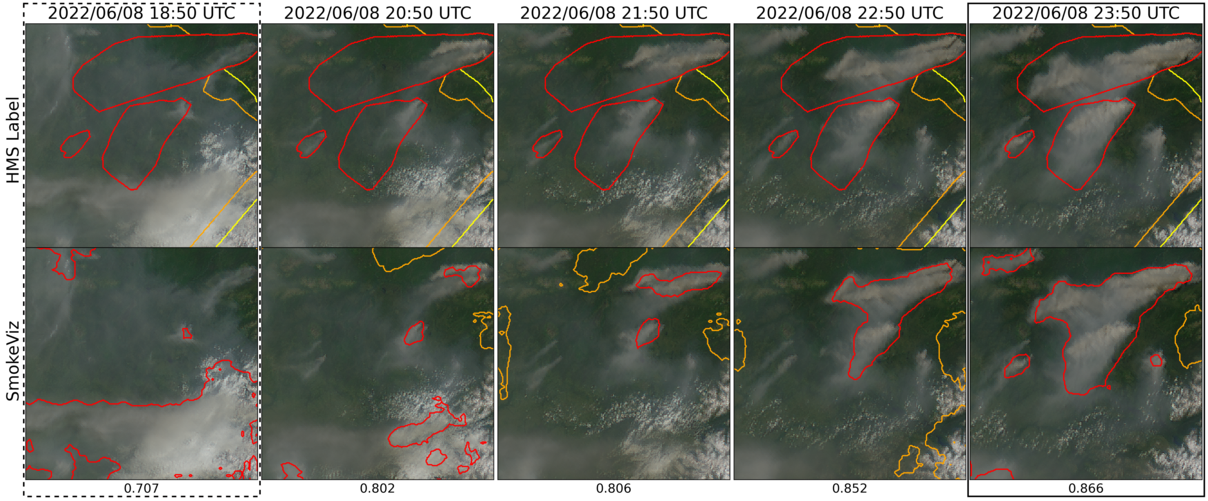
\includegraphics[width=\linewidth]{figures/final_results_small.png}
    \caption{GOES-West imagery showing smoke on June 8th, 2022 in Alaska where, at this geolocation (\(61.06^{\circ}\)N, \(156.12^{\circ}\)W), daylight was between 12:43-7:53 UTC. The HMS smoke annotations (top row) span from 18:50 to 23:50 UTC and are compared to the \(f_{\circ}\) generated pseudo-labels (bottom row). The first column (dotted outline) would be the GOES imagery selected for \(\mathcal{D}_{M}\) since it is closest to sunrise. The last column (solid outline) was selected for \(\mathcal{D}_{p}\) since it had the highest IoU value between the pseudo-label and analyst annotation. The IoU score over all densities is reported at the bottom of each column.}
    \label{ml_vs_mei}
\end{figure*}

An illustration of a pseudo-label picked image better representing the analyst annotation when compared to the Mie-derived image selection is evident in Figure \ref{ml_vs_mei}, where the heavy density smoke IoU increases from 0.01 to 0.59. The analyst annotation for these densities cover 5 hours of imagery, the Mie-derived selection optimizes for the image closest to sunrise while the pseudo-label image selection chooses the image with the highest overlap between the pseudo-label and the analyst annotation. Figure \ref{ml_vs_mei} also illustrates how using a deep learning model can provide higher time resolution and give a dynamic representation of smoke over time.

To get an idea on how \(f_{c}\) compares to the HMS analyst annotations we show a series of samples from \(\mathcal{D}_{p}\) in Figure \ref{bench}. The examples give a qualitative representation of how the predictions from \(f_c\) can provide more detailed boundaries of smoke densities than the HMS annotations do.

\begin{table}[h]
    \caption{Comparison of semantic segmentation model IoU performance on \(\mathcal{D}_{p}\).}\label{bench}
    \centering
    \begin{tabular}{cccrrcrc}
        \toprule
           & DLV3+ & MANet & PSPNet & Linknet \\
        \midrule
        heavy   & 0.411 & 0.336  & 0.355 & 0.324 \\
        medium  & 0.484 & 0.487  & 0.502 & 0.456 \\
        light   & 0.662 & 0.675  & 0.690 & 0.662 \\
        overall & 0.607 & 0.615  & 0.626 & 0.601 \\
        \bottomrule
    \end{tabular}
\end{table}

The results for the benchmarking models (table \ref{bench}) show similar performance across the models. DeepLabV3+ (\(f_c\)) gives the highest heavy density smoke IoU value, while PSPNet gives the highest overall IoU score.

\begin{figure}[!htb]
    \centering
    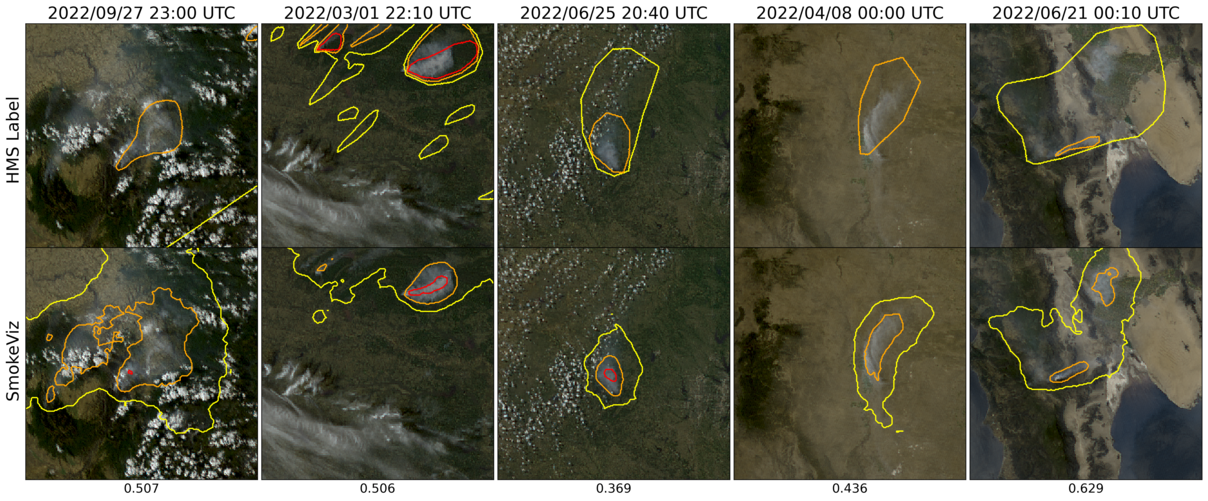
\includegraphics[width=\linewidth]{figures/examples_small.png}
    \caption{Examples of HMS annotations (top row) vs \(f_{c}\) output (bottom row) on \(\mathcal{D}_{p}\) samples. The overall IoU score is reported at the bottom of each column.}\label{examples}
\end{figure}

\section{Limitations}

One of the concerns that comes with using pseudo-labeling methods is that you can perpetuate biases from the parent model into subsequent child models. Due to the increase in detectable forward scattered light off smoke particular matter, we expect the model to have a bias towards producing a higher success rate for smoke detection at larger solar zenith angles. The original HMS annotations do not distinguish by type of fire and include a large representation of controlled agricultural burns. This can be a limitation to consider if the dataset is being trained to target detection of large wildfires. All these limitations are discussed and analyzed further in the Supplementary Materials. Additional work should be done to analyze the performance of SmokeViz derived models on dust vs smoke.

\section{Conclusion}

In this study, we have refined an existing dataset originally curated by NOAA's HMS team, transforming it from a many-to-one imagery-to-annotation format to a more succinct, one-to-one satellite image-to-annotation dataset. The initial HMS dataset provided a general approximation of where smoke had been present for a given time window, though it did not guarantee the actual existence of smoke in the labeled pixels during the given times. Our goal was to create a dataset that could be used, along with additional applications, to train a model to detect wildfire smoke in real-time on an image-by-image level. The Mie-derived dataset selection process determined that if smoke was present, what timestamp within the analyst time window would the give the highest smoke signal-to-noise ratio. While optimizing for being able to detect smoke, if it is present, the Mie-dataset selection had no metric to determine if the smoke was effectually present in the selected image. Since many of the images within the HMS time-window either contained no smoke at all or the smoke was not contained within the geospatial bounds of the annotations, the Mie-derived dataset contained a large number of mislabeled samples. Discrepancies between data and labels can be detrimental towards the model's capacity to improve on feature representations in the target domain. During model training, the penalization of accurate predictions can inadvertently introduce biases towards misclassifying noise as meaningful signal. 

To improve the dataset's capacity to accurately represent wildfire smoke plumes, we train a parent machine learning model, \(f_{\circ}\), using the Mie-derived dataset, \(\mathcal{D}_M\), and run it on the relevant satellite images within the time-frame. The image with the maximum IoU score between the model's smoke predictions, or pseudo-label, and the analyst smoke annotations are used to create the pseudo-label generated dataset, \(\mathcal{D}_{p}\). We then train a child model, \(f_c\), using \(\mathcal{D}_{p}\) and test \(f_{\circ}\) and \(f_c\) on both the 2022 testing sets from \(\mathcal{D}_{M}\) and \(\mathcal{D}_{p}\). The results reported in table \ref{iou_results} suggest that \(\mathcal{D}_{p}\) was able to train a better performing model, \(f_c\), that gave higher IoU metrics on both dataset's testing sets in comparison to the original parent model, \(f_{\circ}\).

The result of this study is a representative dataset, SmokeViz, that can be used to train machine learning models for various wildfire smoke applications. A future goal is to produce a robust and reliable machine learning based approach for detecting wildfires using satellite imagery. That information can be used for wildfire detection and monitoring in along with a highly needed smoke product for data assimilation into smoke dispersion models. Additionally, this dataset can be used as a benchmark for how well remote sensing segmentation models can perform on dispersed edges such as smoke. On a broader scale, we show how pseudo-labeling can be used to optimize a dataset when the resolution for the data and corresponding labels do not match. This could be useful in similar applications involving time-series/video data with a singular label where the data can be compressed while still remaining representative of the label. All data is made publicly available at [aws download link] and all code can be found at \url{https://github.com/anonymous-smokeviz/SmokeViz}.






\bibliography{references}

\end{document}
